% Weights
% Made with Xematics. Positions are in px (1 px = 0.75 pt), as in the SVG export.
\documentclass[tikz, border=4pt]{standalone}
\definecolor{xm1}{HTML}{FFFFFF}
\definecolor{xm2}{HTML}{D4E8F5}
\definecolor{xm3}{HTML}{0072B2}
\definecolor{xm4}{HTML}{F1F2F4}
\definecolor{xm5}{HTML}{4B5563}
\definecolor{xm6}{HTML}{FBE8C4}
\definecolor{xm7}{HTML}{B97800}
\definecolor{xm8}{HTML}{D55E00}
\definecolor{xm9}{HTML}{1F2937}
\definecolor{xm10}{HTML}{6B7280}
\begin{document}
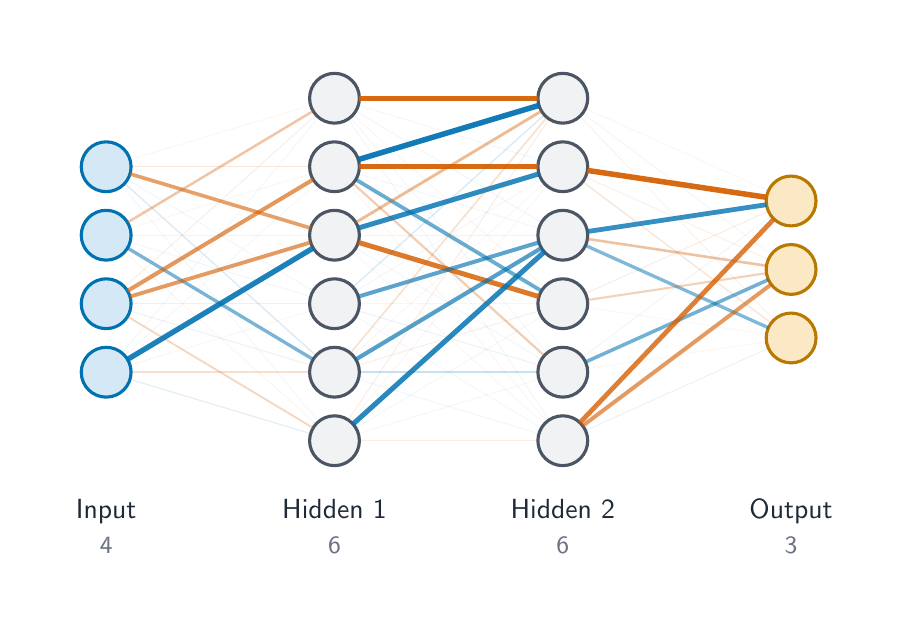
\begin{tikzpicture}[x=0.75pt, y=-0.75pt]
  \tikzset{
    xm input/.style={circle, minimum size=18pt, inner sep=0, outer sep=0, fill=xm2, draw=xm3, line width=1.13pt},
    xm hidden/.style={circle, minimum size=18pt, inner sep=0, outer sep=0, fill=xm4, draw=xm5, line width=1.13pt},
    xm output/.style={circle, minimum size=18pt, inner sep=0, outer sep=0, fill=xm6, draw=xm7, line width=1.13pt},
    xm weight negative/.style={draw=xm8},
    xm weight positive/.style={draw=xm3},
    xm name xm9/.style={text=xm9, inner sep=0, font=\sffamily\fontsize{9.75}{11.7}\selectfont},
    xm size xm10/.style={text=xm10, inner sep=0, font=\sffamily\fontsize{9}{10.8}\selectfont},
  }
  \fill[xm1] (0,0) rectangle (411.07,278.25);
  % Neurons
  \node[xm input] (n-0-0) at (37.82,67) {};
  \node[xm input] (n-0-1) at (37.82,100) {};
  \node[xm input] (n-0-2) at (37.82,133) {};
  \node[xm input] (n-0-3) at (37.82,166) {};
  \node[xm hidden] (n-1-0) at (147.82,34) {};
  \node[xm hidden] (n-1-1) at (147.82,67) {};
  \node[xm hidden] (n-1-2) at (147.82,100) {};
  \node[xm hidden] (n-1-3) at (147.82,133) {};
  \node[xm hidden] (n-1-4) at (147.82,166) {};
  \node[xm hidden] (n-1-5) at (147.82,199) {};
  \node[xm hidden] (n-2-0) at (257.82,34) {};
  \node[xm hidden] (n-2-1) at (257.82,67) {};
  \node[xm hidden] (n-2-2) at (257.82,100) {};
  \node[xm hidden] (n-2-3) at (257.82,133) {};
  \node[xm hidden] (n-2-4) at (257.82,166) {};
  \node[xm hidden] (n-2-5) at (257.82,199) {};
  \node[xm output] (n-3-0) at (367.82,83.5) {};
  \node[xm output] (n-3-1) at (367.82,116.5) {};
  \node[xm output] (n-3-2) at (367.82,149.5) {};
  % Connections 0
  \draw[xm weight negative, line width=0.34pt, opacity=0.05] (n-0-0) -- (n-1-0);
  \draw[xm weight negative, line width=0.52pt, opacity=0.15] (n-0-0) -- (n-1-1);
  \draw[xm weight negative, line width=1.32pt, opacity=0.58] (n-0-0) -- (n-1-2);
  \draw[xm weight positive, line width=0.35pt, opacity=0.06] (n-0-0) -- (n-1-3);
  \draw[xm weight positive, line width=0.5pt, opacity=0.14] (n-0-0) -- (n-1-4);
  \draw[xm weight positive, line width=0.34pt, opacity=0.05] (n-0-0) -- (n-1-5);
  \draw[xm weight negative, line width=0.9pt, opacity=0.35] (n-0-1) -- (n-1-0);
  \draw[xm weight negative, line width=0.34pt, opacity=0.05] (n-0-1) -- (n-1-1);
  \draw[xm weight positive, line width=0.37pt, opacity=0.07] (n-0-1) -- (n-1-2);
  \draw[xm weight positive, line width=0.36pt, opacity=0.06] (n-0-1) -- (n-1-3);
  \draw[xm weight positive, line width=1.22pt, opacity=0.52] (n-0-1) -- (n-1-4);
  \draw[xm weight negative, line width=0.36pt, opacity=0.06] (n-0-1) -- (n-1-5);
  \draw[xm weight negative, line width=0.41pt, opacity=0.09] (n-0-2) -- (n-1-0);
  \draw[xm weight negative, line width=1.45pt, opacity=0.64] (n-0-2) -- (n-1-1);
  \draw[xm weight negative, line width=1.4pt, opacity=0.62] (n-0-2) -- (n-1-2);
  \draw[xm weight positive, line width=0.41pt, opacity=0.09] (n-0-2) -- (n-1-3);
  \draw[xm weight positive, line width=0.41pt, opacity=0.08] (n-0-2) -- (n-1-4);
  \draw[xm weight negative, line width=0.68pt, opacity=0.24] (n-0-2) -- (n-1-5);
  \draw[xm weight positive, line width=0.34pt, opacity=0.05] (n-0-3) -- (n-1-0);
  \draw[xm weight positive, line width=0.34pt, opacity=0.05] (n-0-3) -- (n-1-1);
  \draw[xm weight positive, line width=1.91pt, opacity=0.89] (n-0-3) -- (n-1-2);
  \draw[xm weight negative, line width=0.34pt, opacity=0.05] (n-0-3) -- (n-1-3);
  \draw[xm weight negative, line width=0.59pt, opacity=0.19] (n-0-3) -- (n-1-4);
  \draw[xm weight positive, line width=0.44pt, opacity=0.11] (n-0-3) -- (n-1-5);
  % Connections 1
  \draw[xm weight negative, line width=1.98pt, opacity=0.93] (n-1-0) -- (n-2-0);
  \draw[xm weight positive, line width=0.34pt, opacity=0.05] (n-1-0) -- (n-2-1);
  \draw[xm weight positive, line width=0.35pt, opacity=0.06] (n-1-0) -- (n-2-2);
  \draw[xm weight negative, line width=0.35pt, opacity=0.06] (n-1-0) -- (n-2-3);
  \draw[xm weight positive, line width=0.34pt, opacity=0.05] (n-1-0) -- (n-2-4);
  \draw[xm weight positive, line width=0.35pt, opacity=0.05] (n-1-0) -- (n-2-5);
  \draw[xm weight positive, line width=1.99pt, opacity=0.93] (n-1-1) -- (n-2-0);
  \draw[xm weight negative, line width=1.97pt, opacity=0.92] (n-1-1) -- (n-2-1);
  \draw[xm weight positive, line width=0.34pt, opacity=0.05] (n-1-1) -- (n-2-2);
  \draw[xm weight positive, line width=1.34pt, opacity=0.59] (n-1-1) -- (n-2-3);
  \draw[xm weight negative, line width=0.8pt, opacity=0.3] (n-1-1) -- (n-2-4);
  \draw[xm weight negative, line width=0.34pt, opacity=0.05] (n-1-1) -- (n-2-5);
  \draw[xm weight negative, line width=1.03pt, opacity=0.42] (n-1-2) -- (n-2-0);
  \draw[xm weight positive, line width=1.79pt, opacity=0.82] (n-1-2) -- (n-2-1);
  \draw[xm weight negative, line width=0.42pt, opacity=0.09] (n-1-2) -- (n-2-2);
  \draw[xm weight negative, line width=1.8pt, opacity=0.83] (n-1-2) -- (n-2-3);
  \draw[xm weight positive, line width=0.35pt, opacity=0.05] (n-1-2) -- (n-2-4);
  \draw[xm weight negative, line width=0.34pt, opacity=0.05] (n-1-2) -- (n-2-5);
  \draw[xm weight positive, line width=0.51pt, opacity=0.14] (n-1-3) -- (n-2-0);
  \draw[xm weight positive, line width=0.34pt, opacity=0.05] (n-1-3) -- (n-2-1);
  \draw[xm weight positive, line width=1.45pt, opacity=0.64] (n-1-3) -- (n-2-2);
  \draw[xm weight positive, line width=0.35pt, opacity=0.05] (n-1-3) -- (n-2-3);
  \draw[xm weight positive, line width=0.39pt, opacity=0.08] (n-1-3) -- (n-2-4);
  \draw[xm weight positive, line width=0.34pt, opacity=0.05] (n-1-3) -- (n-2-5);
  \draw[xm weight negative, line width=0.58pt, opacity=0.18] (n-1-4) -- (n-2-0);
  \draw[xm weight negative, line width=0.34pt, opacity=0.05] (n-1-4) -- (n-2-1);
  \draw[xm weight positive, line width=1.5pt, opacity=0.67] (n-1-4) -- (n-2-2);
  \draw[xm weight negative, line width=0.41pt, opacity=0.09] (n-1-4) -- (n-2-3);
  \draw[xm weight positive, line width=0.65pt, opacity=0.22] (n-1-4) -- (n-2-4);
  \draw[xm weight positive, line width=0.35pt, opacity=0.06] (n-1-4) -- (n-2-5);
  \draw[xm weight negative, line width=0.42pt, opacity=0.1] (n-1-5) -- (n-2-0);
  \draw[xm weight negative, line width=0.34pt, opacity=0.05] (n-1-5) -- (n-2-1);
  \draw[xm weight positive, line width=1.82pt, opacity=0.84] (n-1-5) -- (n-2-2);
  \draw[xm weight positive, line width=0.34pt, opacity=0.05] (n-1-5) -- (n-2-3);
  \draw[xm weight negative, line width=0.37pt, opacity=0.06] (n-1-5) -- (n-2-4);
  \draw[xm weight negative, line width=0.45pt, opacity=0.11] (n-1-5) -- (n-2-5);
  % Connections 2
  \draw[xm weight negative, line width=0.34pt, opacity=0.05] (n-2-0) -- (n-3-0);
  \draw[xm weight positive, line width=0.34pt, opacity=0.05] (n-2-0) -- (n-3-1);
  \draw[xm weight negative, line width=0.38pt, opacity=0.07] (n-2-0) -- (n-3-2);
  \draw[xm weight negative, line width=1.99pt, opacity=0.93] (n-2-1) -- (n-3-0);
  \draw[xm weight negative, line width=0.39pt, opacity=0.08] (n-2-1) -- (n-3-1);
  \draw[xm weight negative, line width=0.53pt, opacity=0.15] (n-2-1) -- (n-3-2);
  \draw[xm weight positive, line width=1.73pt, opacity=0.79] (n-2-2) -- (n-3-0);
  \draw[xm weight negative, line width=0.94pt, opacity=0.37] (n-2-2) -- (n-3-1);
  \draw[xm weight positive, line width=1.19pt, opacity=0.5] (n-2-2) -- (n-3-2);
  \draw[xm weight negative, line width=0.42pt, opacity=0.1] (n-2-3) -- (n-3-0);
  \draw[xm weight negative, line width=0.77pt, opacity=0.28] (n-2-3) -- (n-3-1);
  \draw[xm weight negative, line width=0.34pt, opacity=0.05] (n-2-3) -- (n-3-2);
  \draw[xm weight positive, line width=0.36pt, opacity=0.06] (n-2-4) -- (n-3-0);
  \draw[xm weight positive, line width=1.28pt, opacity=0.55] (n-2-4) -- (n-3-1);
  \draw[xm weight negative, line width=0.34pt, opacity=0.05] (n-2-4) -- (n-3-2);
  \draw[xm weight negative, line width=1.72pt, opacity=0.79] (n-2-5) -- (n-3-0);
  \draw[xm weight negative, line width=1.42pt, opacity=0.62] (n-2-5) -- (n-3-1);
  \draw[xm weight positive, line width=0.4pt, opacity=0.08] (n-2-5) -- (n-3-2);
  % Labels
  \node[xm name xm9, anchor=base] at (37.82,236.59) {Input};
  \node[xm size xm10, anchor=base] at (37.82,253.35) {4};
  \node[xm name xm9, anchor=base] at (147.82,236.59) {Hidden 1};
  \node[xm size xm10, anchor=base] at (147.82,253.35) {6};
  \node[xm name xm9, anchor=base] at (257.82,236.59) {Hidden 2};
  \node[xm size xm10, anchor=base] at (257.82,253.35) {6};
  \node[xm name xm9, anchor=base] at (367.82,236.59) {Output};
  \node[xm size xm10, anchor=base] at (367.82,253.35) {3};
\end{tikzpicture}
\end{document}
